\documentclass[a4paper,11pt]{ltjsarticle}

% Utility packages
\usepackage{graphicx} % For images
\usepackage{amsmath, amssymb} % For math
\usepackage{url} % For URLs
\usepackage[hidelinks]{hyperref} % For hyperlinks
\usepackage{booktabs} % For nice tables
\usepackage{longtable} % For long tables
\usepackage{float} % For H placement
\usepackage{tikz}
\usetikzlibrary{shapes, arrows, positioning, shapes.geometric, shadows}
\usepackage{listings} % For code listing
\usepackage{xcolor} % For colors

% Define Markdown-like listing style
\definecolor{codegray}{rgb}{0.95,0.95,0.95}
\lstdefinestyle{markdown}{
    backgroundcolor=\color{codegray},
    basicstyle=\ttfamily\small,
    breaklines=true,
    frame=none,
    keepspaces=true,
    showspaces=false,
    showstringspaces=false,
    showtabs=false,
    tabsize=2,
    columns=fullflexible,
    xleftmargin=1em,
    xrightmargin=1em,
    aboveskip=1em,
    belowskip=1em,
    framesep=0.5em,
    frame=single,
    rulecolor=\color{codegray},
    framerule=0pt
}
\lstset{style=markdown}


\begin{document}

\begin{titlepage}
    \begin{center}
        \vspace*{1cm}
        
        {\Large 九州大学大学院理学府 \par}
        {\Large 地球惑星科学専攻 \par}
        {\Large 修士論文 \par}
        
        \vspace{3cm}
        
        {\Huge EE-indexを用いた特異型EEJの発生特性の解明 \par}
        \vspace{0.5cm}
        {\Large (宇宙天気データベースシステムの開発に向けて) \par}
        
        \vspace{2cm}
        
        {\Large Elucidation of the occurrence characteristics of peculiar EEJ using the EE-index \par}
        \vspace{0.5cm}
        {\Large Towards the Development of a Space Weather Database System~ \par}
        
        \vspace{3cm}
        
        {\Large 2SC24221P \par}
        {\Large 宇宙地球電磁気学研究分野 \par}
        {\Large 菊池 裕夢 \par}        
        
    \end{center}
\end{titlepage}

\tableofcontents
\clearpage

\section*{要旨}
ここに要旨を書く。

\clearpage

\section{序論}
\subsection{研究背景}

\subsection{特異型EEJ研究の現状と課題}

\subsection{本研究の目的}

\subsection{本論文の構成}


\section{導入}
\subsection{MAGDAS観測網の概要}
MAGDASとは、九州大学国際宇宙惑星環境研究センターを中心に運用されている、世界最大規模の地上多点地磁気観測ネットワークである。
磁気赤道および磁気子午線210$^\circ$に沿って南北半球に磁力計とデータ収集システムを高密度に配置し、観測された磁場データはリアルタイムで送信されている。
これにより、地磁気主磁場とダイナモ作用に起因するSq場などの全球的磁場現象について、その緯度構造や長期・短期変動を解析することが可能である(図\ref{fig:magdas_network})。


\begin{figure}[htbp]
    \centering
    \includegraphics[width=0.8\textwidth]{figures/magdas_network.png}
    \caption{MAGDAS観測網}
    \label{fig:magdas_network}
\end{figure}

%!TEX root = ../../main.tex
\subsection{INTERMAGNETおよびTTBデータ}

INTERMAGNET (International Real-time Magnetic Observatory Network) は,地球磁場の変動をリアルタイムかつ高精度に監視し,データを提供することを目的とした国際的な地磁気観測所ネットワークである.
1980年代後半に設立され,世界各国の研究機関や大学が参加している.
INTERMAGNETに参加する観測所 (IMO: International Magnetic Observatory) は,測定機器やデータ処理に関して厳格な技術標準を遵守しており,これによりデータの品質と互換性が保たれている.
観測データは,標準的なデータ交換フォーマットであるIAGA-2002形式などで記録され,地域のGIN (Geomagnetic Information Node) と呼ばれるデータセンターに集約された後,科学コミュニティや商業利用のために公開されている.

本研究において解析対象とするTTBデータは,INTERMAGNETの観測所であるブラジルのTatuoca観測所 (IAGAコード: TTB) で取得されたものである.(表\ref{tab:ttb_station})
この観測所は磁気赤道の非常に近くに位置しているため,昼側の磁気赤道上空の電離圏E層を流れる強力な電流系である赤道ジェット電流 (Equatorial Electrojet: EEJ) の影響を直接的に観測することができる.
そのため,TTBデータはEEJの強度変動やその構造を研究する上で極めて重要な指標となる.
INTERMAGNETの高品質なデータ標準により,微細な磁場変動の解析や長期的な傾向の把握が可能となっている.

\begin{table}[htbp]
  \centering
  \caption{Tatuoca (TTB) 観測所の詳細}
  \label{tab:ttb_station}
  \begin{tabular}{llrrr}
    \toprule
    Code & Name & GG.Lat & GG.Lon  & Dip.Lat \\
    \midrule
    TTB & Tatuoca & -1.23 & -48.51 & -0.72 \\
    \bottomrule
  \end{tabular}
\end{table}

\subsection{地磁気日変化とSq電流}

\subsection{赤道ジェット電流(EEJ)}
磁気赤道域で観測される地上磁場変動において、最も優勢な現象が赤道ジェット電流(Equatorial ElectroJet: EEJ)によるものである。
EEJは昼側の磁気赤道電離圏を東向きに流れる電流で、それによるH成分の磁場変動は最大で$+200$\,nT程度にもなる。
一方、西向きのジェット電流によってH成分が減少する変動も見られる。
これは赤道カウンタージェット電流(Equatorial Counter ElectroJet: CEJ)と呼ばれている。
CEJによる磁場変動は明け方や夕方に見られることが多い。

磁気赤道域電離圏特有のカウリング効果(Cowling Effect)がある。
これは、赤道域では地球の磁力線が地平に対して水平になることから生まれる効果である。
カウリング効果は磁気赤道を中心に非常に狭い緯度範囲でしか効かないため、EEJやCEJが流れるのも磁気緯度で$\pm 3$度以内の範囲だと言われている。

EEJやCEJが流れるためには電離圏電気伝導度が高いことに加え、外部から電場が印加される必要がある。
太陽風と磁気圏の相互作用で生まれる電場(太陽風中電場)の他にも、電離圏のプラズマと中性大気の相互作用によって大気が太陽によって温められて膨張し、最も温められる赤道正午付近から放射状に流れ出す際、プラズマを引きずりながら磁力線の間を移動することによって生じる。
荷電粒子が磁場の中を移動することで起電力が生じ、この起電力によって北半球では反時計回り、南半球では時計回りの電流系(Sq電流系)が形成される。
Sq電流系は中緯度での磁場の日変化パターンを作る主要な要素である。
ダイナモ電場によって朝側にはプラス、夕側にはマイナスのチャージが溜まる。このチャージによって東向きの電場が磁気赤道域に印加される。
EEJやCEJの変動を注視することで、磁気赤道電離圏や電離圏・大気圏相互作用の状態を監視することが可能である。

\subsection{磁気赤道域における潮汐効果の関係}


\section{EE-index}
\subsection{EE-indexの定義}
EE-indexは、磁気赤道付近の短期的・長期的な変動をリアルタイムでモニターすることを目的として九州大学が提案した新しい地磁気指標である \cite{Uozumi2008}。
EE-indexの算出には磁気赤道域MAGDAS観測点のデータが使用される。
MAGDASには、観測したデータをリアルタイムで転送するシステムが備わっているため、磁気赤道域で観測されたデータをすぐに解析指数化し、その時々の宙空の状態を速報することが可能である。
EE-indexはEDstとEUELの2つの指数から構成される。
EDstはグローバルな擾乱成分でDstの代用として利用することが出来る。
EUELは特定の地点でのみ変動するローカルな擾乱成分を指す。
EUは東向きのローカルな等価電流、ELは西向きのローカルな電流による変動に相当する。
これらの指数を算出することで赤道域の磁気擾乱のスケールの定量化が可能になる。

\subsection{EE-index算出に用いるデータ}

EE-indexの算出には、九州大学が中心となって運用しているMAGDASプロジェクトの磁力計ネットワーク観測データを用いて行う。
本研究で使用する観測点の一覧を表\ref{tab:ee_index_stations}に示す。

\begin{longtable}{ll r r r r r}
    \caption{EE-index算出に使用する観測点一覧}
    \label{tab:ee_index_stations} \\
    \toprule
    Code & Name & GG.Lat & GG.Lon & GM.Lat & GM.Lon & Dip.Lat \\
    \midrule
    \endfirsthead

    \toprule
    Code & Name & GG.Lat & GG.Lon & GM.Lat & GM.Lon & Dip.Lat \\
    \midrule
    \endhead

    \bottomrule
    \endfoot

    AAB & Addis Ababa & 9.04 & 38.77 & 5.41 & 112.54 & 1.21 \\
    ABU & Abuja & 8.99 & 7.39 & -0.54 & 81.31 & -3.36 \\
    AMA & Amami Oshima & 28.17 & 129.33 & 21.11 & 200.88 & 23.39 \\
    ANC & Ancon & -11.77 & -77.15 & -2.11 & 355.57 & 0.13 \\
    BCL & Bac Lieu & 9.32 & 105.71 & -0.36 & 178.36 & 2.50 \\
    BKL & Bengkulu & -3.80 & 102.31 & -15.13 & 173.60 & -13.64 \\
    CDO & Cagayan De Oro & 8.46 & 124.63 & -0.80 & 197.06 & 1.41 \\
    CEB & Cebu & 10.36 & 123.91 & 1.06 & 196.26 & 3.59 \\
    DAV & Davao & 7.00 & 125.40 & -2.22 & 197.90 & -0.27 \\
    DAW & Darwin & -12.41 & 130.92 & -21.91 & 202.81 & -22.40 \\
    EUS & Eusebio & -3.88 & -38.43 & 4.14 & 34.21 & -9.41 \\
    EWA & Ewa Beach & 21.32 & -158.00 & 21.63 & 269.45 & 21.37 \\
    GSI & Gunung Sitoli & 1.30 & 97.58 & -8.25 & 170.10 & -7.65 \\
    HLN & Hualien & 23.90 & 121.55 & 16.86 & 193.05 & 19.37 \\
    HUA & Huancayo & -12.02 & -75.29 & -2.34 & 357.39 & -0.17 \\
    ICA & Ica & -14.09 & -75.74 & -4.42 & 356.97 & -2.07 \\
    ILR & Ilorin & 8.50 & 4.68 & 10.50 & 78.90 & -4.16 \\
    KRT & Khartoum & 15.33 & 32.32 & 12.64 & 107.27 & 7.91 \\
    LAG & Lagos & 6.48 & 3.27 & -3.04 & 75.33 & -6.93 \\
    LGZ & Legazpi & 13.15 & 123.74 & 3.84 & 195.96 & 6.76 \\
    LKW & Langkawi & 6.30 & 99.78 & -3.30 & 172.44 & -1.41 \\
    LWA & Liwa & -5.02 & 104.06 & -16.19 & 175.33 & -14.99 \\
    MND & Manado & 1.44 & 124.84 & -7.80 & 197.63 & -6.50 \\
    MUT & Muntinlupa & 14.37 & 121.02 & 4.95 & 193.26 & 8.32 \\
    NAB & Nairobi & -1.16 & 36.48 & -10.65 & 108.18 & -12.23 \\
    PRP & Pare Pare & -3.60 & 119.40 & -12.38 & 190.75 & -12.23 \\
    SCN & Sicincin & -0.55 & 100.30 & -10.16 & 172.81 & -9.78 \\
    TGG & Tuguegarao & 17.66 & 121.76 & 10.26 & 193.05 & 12.06 \\
    TIR & Tirunelveli & 8.70 & 77.80 & 0.25 & 150.80 & 1.74 \\
    YAP & Yap Island & 9.50 & 138.08 & 1.14 & 210.25 & 1.97 \\
\end{longtable}

\subsection{EE-indexの算出方法}

EE-indexの算出には、磁気赤道域に設置された観測点で得られた地磁気水平成分(H成分)のデータを用いる。
まず、各観測点$s$におけるH成分$B_{H,s}$について、1日間のデータの中央値を基準値(ゼロレベル)として定義し、その基準値からの偏差を$ER_s$とする。
$ER_s$は以下の式で表される。

\begin{equation}
  ER_s(t) = B_{H,s}(t) - \text{median}(B_{H,s})_{\text{1day}}
\end{equation}

ここで、$t$は時刻を表す。
次に、全球的な擾乱成分であるEDst(Equatorial Disturbance storm time)を算出する。
赤道域の夜側(一般に18:00 - 06:00 LT)では、電離圏の電気伝導度が昼側に比べて著しく低下するため、電離圏起源の局所的な電流系による磁場変動は無視できる程度となる。
したがって、夜側に位置する観測点の磁場変動は、主にリングカレントや磁気圏界面電流といった全球的な磁気圏起源の変動を反映していると考えられる。
そこで、夜側(18:00 - 06:00 LT)に位置する全観測点の$ER_s$の平均値をとり、これをEDstと定義する。

\begin{equation}
  EDst(t) = \frac{1}{N_{night}} \sum_{s \in \text{Night}} ER_s(t)
\end{equation}

ここで、$N_{night}$は当該時刻において夜側に位置する観測点の総数である。

最後に、各観測点の$ER_s$からこのEDstを差し引くことで、全球的な変動成分を除去し、局所的な変動成分(主にEEJやSq電流に起因するもの)を抽出する。

\begin{equation}
  \text{EUEL}_s(t) = ER_s(t) - EDst(t)
\end{equation}

これにより、観測点直上の電離圏電流に起因する磁場変動成分を定量的に評価することが可能となる。


\subsection{EE-index精度向上方法}

Uozumi et al. (2008) \cite{Uozumi2008} は、MAGDAS/CPMN観測網のリアルタイムデータを用いて、赤道ジェット電流(EEJ)の短期的および長期的な変動を監視するための新しい指標としてEE-indexを提案した。
この初期の手法では、磁気赤道域の夜側(18-06 LT)にある観測点の水平成分磁場変動の平均値をEDst(Equatorial Disturbance in Storm Time)として定義していた。
EDstはDst指数の代替として機能し、各観測点のH成分からEDstを差し引くことで、局所的なEEJ成分(EU)およびカウンターエレクトロジェット(CEJ)成分(EL)を抽出することが可能である。
しかし、初期の研究段階では利用可能な夜側観測点の数が限られており、EDstの算出精度が観測点配置の制約を受けるという課題があった。

これに対し、Fujimoto et al. (2016) \cite{Fujimoto2016} では、長期的なEEJ変動解析に耐えうるよう、EE-indexに更なる改良が加えられた。
主な改良点は、EDstの算出に使用する観測点数の増加と、緯度補正の導入である。

改良版では、全経度をカバーする観測点を使用することで、より高精度に全球的な変動を見積もることが可能となった。
また、太平洋地域など赤道直下に観測点が存在しない経度帯における精度向上のため、低緯度観測点(磁気緯度$\pm 25^\circ$以内)のデータを用いて赤道上の磁場強度を推定する手法が導入された。
具体的には、観測された水平成分磁場$H_{obs}$と磁気緯度$\Phi$を用いて、赤道上の磁場強度$H_{dip}$を以下の式で推定する。

\begin{equation}
    H_{dip} = \frac{H_{obs}}{\cos \Phi}
\end{equation}

この補正により、赤道直下に観測点がない経度でも、近隣の低緯度観測点からEDstの算出に必要なデータを補完することが可能となり、EDstの算出精度が向上した。
これらの改良により、EE-indexは地磁気静穏時だけでなく、磁気嵐時などの地磁気擾乱時においても、赤道域の磁場変動を定量的に評価できる指標となっている。


\section{特異型EEJと自動判定の手法}
\subsection{特異型EEJとは}

\subsection{未発達型・突発型}

\subsection{特異型EEJの自動判定の手法}
ここに結果1を書く。


\section{結果: 特異型EEJの発生特性}
\subsection{解析条件および対象期間}

\subsection{南米領域(ペルー・ブラジル)の解析結果}
ここに結果2を書く。

\subsection{ブラジル領域における解析結果}


\section{考察}
\subsection{南米領域における特異型EEJ発生要因}

\subsection{季節依存性との関連性}

\subsection{潮汐効果との関連性}


\section{宇宙天気データベースシステムへの応用}
\subsection{システム開発の目的}
本章では、宇宙天気データベースシステムの開発について述べる。
システム開発の主な目的は、以下の3点である。
第一に、近年高まりを見せる宇宙天気のリアルタイム監視への需要に応えることである。
第二に、本研究で算出されるEE-indexを広く研究者コミュニティ等へ公開することである。
そして第三に、本研究で構築した手法を用いて特異型EEJをリアルタイムで検知する機能を実装することである。
迅速な状況把握とデータ共有は、宇宙天気予報の精度向上や関連研究の発展に寄与するものであり、本システムはその基盤を提供するものである。

\subsection{システム全体構成}
本章では、本システムの全体構成および採用した技術スタックについて述べる。

\subsubsection{全体構成とリポジトリ運用の工夫}
本システムの開発プロジェクトは、フロントエンドとバックエンドを単一のリポジトリで管理するモノレポ(Monorepo)構成を採用している。
図\ref{fig:system_architecture}にシステムの全体構成図を示す。
ユーザーはWebブラウザを通じてシステムにアクセスし、フロントエンドがバックエンドのAPIを利用してMAGDAS観測データを取得・表示する構成となっている。

\begin{figure}[H]
  \centering
  \resizebox{\textwidth}{!}{
    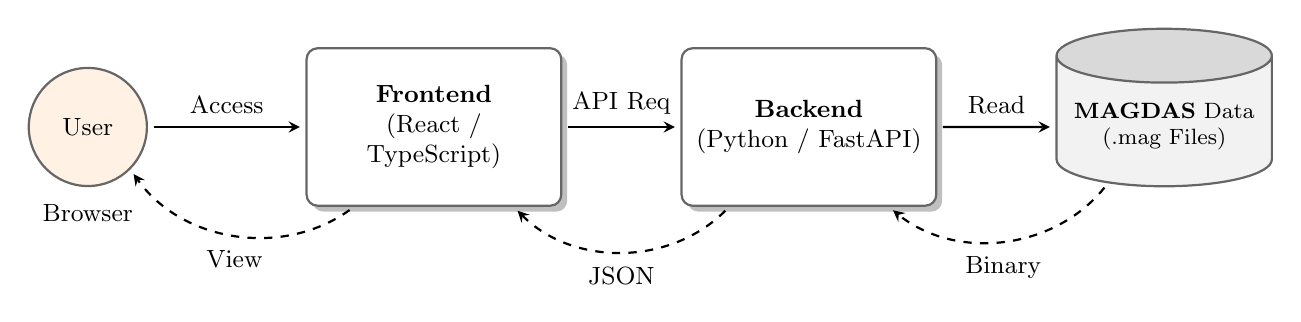
\begin{tikzpicture}[
        node distance=1.0cm,
        auto,
        font=\small,
        % Styles
        component/.style={
            rectangle,
            draw=black!60,
            thick,
            fill=white,
            text width=3.0cm,
            align=center,
            rounded corners,
            minimum height=2.0cm,
            drop shadow
          },
        database/.style={
            cylinder,
            cylinder uses custom fill,
            cylinder body fill=gray!10,
            cylinder end fill=gray!30,
            shape border rotate=90,
            aspect=0.25,
            draw=black!60,
            thick,
            text width=2.5cm,
            align=center,
            font=\footnotesize,
            minimum height=2.0cm,
            minimum width=2.0cm
          },
        user/.style={
            circle,
            draw=black!60,
            thick,
            fill=orange!10,
            minimum size=1.5cm,
            align=center
          },
        arrow/.style={
            ->,
            >=stealth,
            thick,
            shorten <=2pt,
            shorten >=2pt
          }
      ]
      % Nodes
      % User Node (Left)
      \node[user] (user) {User};
      \node[below=0.1cm of user] {Browser};

      % Frontend Node
      \node[component, right=2.0cm of user] (frontend) {\textbf{Frontend} \\ (React / TypeScript)};

      % Backend Node
      \node[component, right=1.5cm of frontend] (backend) {\textbf{Backend} \\ (Python / FastAPI)};

      % Database Node (Right)
      \node[database, right=1.5cm of backend] (data) {\textbf{\mbox{MAGDAS}} Data \\ (.mag Files)};

      % Arrows (Interaction Flow)
      \draw[arrow] (user) -- node[midway, above, yshift=1pt] {Access} (frontend);
      \draw[arrow] (frontend) -- node[midway, above, yshift=1pt] {API Req} (backend);
      \draw[arrow] (backend) -- node[midway, above, yshift=1pt] {Read} (data);

      % Return Arrows (Data Flow)
      \draw[arrow, dashed, bend left=45] (data) to node[midway, below, yshift=-2pt] {Binary} (backend);
      \draw[arrow, dashed, bend left=45] (backend) to node[midway, below, yshift=-2pt] {JSON} (frontend);
      \draw[arrow, dashed, bend left=45] (frontend) to node[midway, below, yshift=-2pt] {View} (user);

    \end{tikzpicture}
  }
  \caption{システム全体構成図}
  \label{fig:system_architecture}
\end{figure}

また、本研究ではシステム開発としての品質維持と、研究活動としての柔軟な試行錯誤を両立させる必要がある。
そのため、プロジェクト内に`dev`ディレクトリを設け、研究目的の実験的なコードや解析アルゴリズムのプロトタイプ実装はここに配置する運用とした。
これにより、研究開発のスピードを落とすことなく、本番稼働システムのコードベースをクリーンに保つことが可能となっている。

\subsubsection{バックエンド設計}
バックエンドの実装においては、保守性と拡張性を高めるため、レイヤードアーキテクチャを採用し、責務を以下の4層に分離している。

\begin{itemize}
  \item \textbf{Handler層}: クライアントからのHTTPリクエストを受け付け、Usecase層へ処理を委譲し、その結果をレスポンスとして返却する。
  \item \textbf{Usecase層}: アプリケーション固有のビジネスロジックを実装し、具体的な処理の流れを制御する。
  \item \textbf{Service層}: 数値計算やデータ加工などのドメイン固有の計算処理(ビジネスロジック)を担当する。本層で実装されたロジックは、本番稼働システムだけでなく、前述の`dev`層での統計解析においても共通して利用される。これにより、研究成果をスムーズにシステムへ反映することが可能となっている。
  \item \textbf{Repository層}: データソース(ファイルシステム上の.magファイル)へのアクセスを抽象化し、データの取得処理を一元管理する。
\end{itemize}

\subsubsection{技術スタック}
本システムの開発および運用環境として、以下の技術スタックを選定した。

\begin{itemize}
  \item \textbf{バックエンド}: Python, FastAPI
  \item \textbf{フロントエンド}: TypeScript, React, Tailwind CSS
  \item \textbf{データベース (データソース)}: 研究室サーバー上の.magファイル (独自フォーマット)
  \item \textbf{実行環境}: オンプレミスサーバー
\end{itemize}

バックエンドにPython (FastAPI) を採用した主な理由は、数値計算ライブラリが充実しており、システム開発と並行してデータ解析を効率的に行える点にある。
Pythonは科学技術計算の分野で広く利用されており、本研究においてもデータの一次処理や解析アルゴリズムの実装に適している。
また、Matplotlib等の描画ライブラリが豊富であるため、解析結果の可視化や検証も円滑に行うことができ、研究活動とシステム開発の相互運用性を高める上で最適な選択であるといえる。

%\subsection{技術スタック}
本システムの開発および運用環境として、以下の技術スタックを選定した。
システムはオンプレミス環境で動作し、研究室のサーバー内に蓄積されたデータを活用する構成となっている。

\begin{itemize}
    \item \textbf{バックエンド}: Python, FastAPI
    \item \textbf{フロントエンド}: TypeScript, React
    \item \textbf{データベース (データソース)}: 研究室サーバー上の.magファイル (独自フォーマット)
    \item \textbf{実行環境}: オンプレミスサーバー
\end{itemize}

バックエンドにPython (FastAPI) を採用した主な理由は、数値計算ライブラリが充実しており、システム開発と並行してデータ解析を効率的に行える点にある。
Pythonは科学技術計算の分野で広く利用されており、本研究においてもデータの一次処理や解析アルゴリズムの実装に適している。
また、Matplotlib等の描画ライブラリが豊富であるため、解析結果の可視化や検証も円滑に行うことができ、研究活動とシステム開発の相互運用性を高める上で最適な選択であるといえる。

フロントエンドには、モダンなUI構築と保守性を重視し、TypeScriptおよびReactを使用している。
また、データの永続化・管理手法としては、既存の研究室サーバーに蓄積されているMAGDAS観測網のバイナリデータ(.magファイル)を直接読み込み、APIを通じてフロントエンドへ提供する形態をとっている。
 % Merged into architecture.tex
\subsection{開発手法}
本研究におけるシステム開発では、効率性と品質を担保するために、モダンな開発フローとツールチェーンを採用している。
具体的には、バージョン管理システムによるソースコード管理、パッケージマネージャーによる依存関係の解決、そしてMakefileによるタスクの自動化を行っている。
また、開発環境と本番環境の乖離を防ぐため、Dockerコンテナ技術を積極的に活用している。
詳細な環境構築手順および運用方法については、次節「\ref{sec:system_setup} 環境構築・ドキュメント」にて詳述する。

\subsection{環境構築・ドキュメント}
\label{sec:system_setup}
本プロジェクトでは、macOS環境での開発を前提とし、以下の手順で開発環境を構築する。
なお、本節に記載する情報は2026年2月時点のものである。
macOS におけるパッケージ管理を簡便に行うため、各種開発ツールのインストールには Homebrew の利用を推奨する。

\subsubsection{必要なツールのインストール}
まず、以下の開発ツールを導入する。

\begin{itemize}
    \item \textbf{Homebrew}: macOSのパッケージ管理ツール。
    \item \textbf{Git}: ソースコード管理ツール。
    \item \textbf{Docker}: コンテナ仮想化プラットフォーム。
    \item \textbf{uv}: 高速なPythonパッケージマネージャー(バックエンド用)。
    \item \textbf{Node.js}: JavaScript実行環境(フロントエンド用)。
\end{itemize}

\subsubsection{プロジェクトのセットアップ}
リポジトリをクローンした後、プロジェクトルートで以下のコマンドを実行することで、初期セットアップが完了する。

\begin{lstlisting}
git clone https://github.com/kikudesuyo/magdas
cd magdas
make init
\end{lstlisting}

\texttt{make init}コマンドにより、バックエンドの依存ライブラリ(\texttt{uv sync})およびフロントエンドの依存ライブラリ(\texttt{npm install})が一括でインストールされる。

\subsubsection{データ管理}
解析用の観測データ(.mgdファイル等)はリポジトリには含めず、ローカル環境の\texttt{backend/Storage}ディレクトリに個別に配置する運用としている。
これにより、機密性の高いデータや容量の大きなデータをGit管理から除外しつつ、開発環境で本番同様の解析フローを再現することを可能にしている。

\subsubsection{アプリケーションの起動}
開発時のアプリケーション起動方法は、以下の2パターンを用意している。

\begin{enumerate}
    \item \textbf{Dockerでの一括起動(推奨)}: \\
    \texttt{make up}コマンドを実行することで、バックエンドとフロントエンドをコンテナとして一括起動する。実環境との差異が少なく、手軽に動作確認を行うことが可能である。
    コンテナ起動後は、以下のURLでアクセス可能となる。
    \begin{itemize}
        \item フロントエンド: \url{http://localhost:5173}
        \item バックエンドAPI: \url{http://localhost:8000}
    \end{itemize}

    \item \textbf{ローカルでの個別起動}: \\
    デバッグ等の目的で、各サービスを個別に起動する場合に使用する。

    \textbf{バックエンド起動}:
\begin{lstlisting}
make be-dev
\end{lstlisting}

    \textbf{フロントエンド起動}:
\begin{lstlisting}
make fe-dev
\end{lstlisting}
\end{enumerate}

\subsection{今後の課題}
2026年2月現在、本システムにはパフォーマンスおよびスケーラビリティ、開発プロセスの観点でいくつかの課題が残されている。
主な課題は以下の3点である。

\begin{enumerate}
    \item \textbf{EE-index算出処理の効率化} \\
    EE-indexの算出結果は入力データが同一であれば常に同じ値となる(冪等性を持つ)にもかかわらず、本システムではリクエストの度に毎回算出処理を行っている。これにより、レスポンスタイムが著しく遅延する原因となっているため、計算結果の再利用が求められる。

    \item \textbf{データ管理とキャッシュ機構の導入} \\
    現状ではデータベースマネジメントシステムを使用せず、ファイルシステム上のデータを直接読み込んで処理を行っている。また、頻繁にアクセスされるデータに対するキャッシュ機構も導入されていない。今後トラフィックが増加した場合、サーバー負荷の増大や応答速度の低下が懸念されるため、効率的なデータ管理基盤の構築が必要である。

    \item \textbf{CI/CD環境の整備} \\
    現状、オンプレミス環境へのデプロイ作業は手動で行われており、更新のたびに手間とリスクが伴う。システムの安定稼働と迅速な機能改善を実現するためには、コードの変更を検知し、自動でビルド・テスト・デプロイを行うCI/CD(継続的インテグレーション・継続的デリバリー)環境の構築が不可欠である。
\end{enumerate}


\section{総括}
ここに総括を書く。


\bibliographystyle{unsrt}
\bibliography{bibliography/references}

\end{document}
